% TODO:
%
% Spell check



\begin{refsection}


\renewcommand{\t}[1]{\texttt{#1}}
\newcommand{\TCB}[1]{\textsf{TCB}(#1)}
\newcommand{\diff}[2]{\textsf{diff}(#1,#2)}

\newcommand{\viF}  {V1-FIO}
\newcommand{\viN}  {V1-NoFIO}
\newcommand{\viiF} {V2-FIO}
\newcommand{\viiN} {V2-NoFIO}
\newcommand{\viiNm}{V2-NoFIO-minTCB}

\newcommand{\emphasize}[1]{{\color{red}\underline{#1}}}

\newenvironment{fbstart}
  {\VerbatimEnvironment\[\begin{minipage}{\textwidth}\begin{minted}[linenos, numbersep=6pt, firstnumber=1]{haskell}}
  {\end{minted}\end{minipage}\]}
\newenvironment{fb}
  {\VerbatimEnvironment\[\begin{minipage}{\textwidth}\begin{minted}[linenos, numbersep=6pt, firstnumber=last]{haskell}}
  {\end{minted}\end{minipage}\]}


\section{Research questions}

An important goal for achieving security is to minimize the size of the \textit{\underline{t}rusted \underline{c}omputing \underline{b}ase} (TCB),
which is the portion of code that must be carefully audited for security \cite{schroeder1975engineering}.
%
(We refer to the remaining code as the \textit{\underline{u}ntrusted \underline{c}omputing \underline{b}ase} (UCB).)

Our hypothesis is that faceted execution (as implemented by the FIO library)
makes it \textit{easier} to minimize the size of the TCB in realistic applications.
%
In particular, we have two research questions:
\begin{enumerate}
  \item
    Does FIO help minimize TCB size when coding a secure application?
  \item
    Does FIO help minimize TCB size when changing an existing application to meet new requirements?
\end{enumerate}
Our experimental design to investigate these questions is as follows:
\begin{itemize}
  \item
    Create Design V1 for a prototype application called \myapp{}.
  \item
    Create Implementation \viF{} using FIO, minimizing the TCB.
  \item
    Create Implementation \viN{} without FIO, minimizing the TCB.
  \item
    Measure TCB size of the two implementations.
  \item
    Create Design V2 by making a small change to Design V1.
  \item
    Create Implementation \viiF{} by modifying \viF{}.
  \item
    Create Implementation \viiN{} by modifying \viN{}.
  \item
    Create Implementation \viiNm{} from \viiN{} by minimizing the TCB.
  \item
    Quantify the effect on security by comparing the increase in TCB size when going from V1 to V2.
  \item
    Quantify the \textit{ease} of achieving security by comparing the number of lines of code changed when minimizing the TCB size in V2.
\end{itemize}
Table \ref{table_loc} shows the number of lines of code for each version.
%
Table \ref{table_diffs} shows the number of edit actions required to change each version to the next.
\begin{table}
\begin{center}
\begin{tabular}{lrrrl}
  &
    \multicolumn{3}{c}{Lines of code}
\\\cline{2-4}
    Version
  &
    FIO
  &
    TCB
  &
    UCB
  &
    Total application-specific code
\\\hline
    \viF{}
  &
    108
  &
    \emphasize{99}
  &
    352
  &
    451
\\
    \viiF{}
  &
    108
  &
    99
  &
    360
  &
    459
\\\hline
    \viN{}
  &
    0
  &
    \emphasize{118}
  &
    295
  &
    413
\\
    \viiN{}
  &
    0
  &
    419
  &
    0
  &
    419
\\
    \viiNm{}
  &
    0
  &
    \emphasize{128}
  &
    298
  &
    426
\\\hline
\end{tabular}
\end{center}
\caption[Number of lines of code in each version of \myapp{}.]{%
The number of lines of code in each version of \myapp{}.
The emphasized entries are useful for quantifying security.%
}
\label{table_loc}
\end{table}
\begin{table}
\begin{center}
\begin{tabular}{lrrrr}
  &
    \multicolumn{4}{c}{Changes (measured in lines of code)}
\\\cline{2-5}
    Version
  &
    Modified
  &
    Moved
  &
    Inserted
  &
    Deleted
\\\hline
    \viF{}
  &
  &
  &
  &
\\
    \viiF{}
  &
    1
  &
    0
  &
    8
  &
    0
\\\hline
    \viN{}
  &
  &
  &
  &
\\
    \viiN{}
  &
    2
  &
    3
  &
    6
  &
    0
\\
    \viiNm{}
  &
    \emphasize{4}
  &
    \emphasize{6}
  &
    \emphasize{7}
  &
    \emphasize{0}
\\\hline
\end{tabular}
\end{center}
\caption[Differences between each version of \myapp{}.]{%
The differences between each version of \myapp{}.
Each row in the table lists the differences from the version in the row above it.
The emphasized entries are useful for quantifying \textit{ease} of achieving security.%
}
\label{table_diffs}
\end{table}
The full source code is available at \url{https://github.com/tommy-schmitz/facetbook}.
%
In the sections below, we discuss these results.

\iffalse

By comparing $1_F$ and $1_N$,
we get a basic understanding of how FIO affects the design of a codebase.

To quantitatively compare confidence in security,
we can compare the size of $\TCB{1_F}$ with the size of $\TCB{1_N}$;
in symbols, we can compare $|\TCB{1_F}|$ with $|\TCB{1_N}|$.
%
However, $\TCB{1_F}$ includes the FIO library itself,
whereas $\TCB{1_N}$ does not,
so the result of the comparison depends heavily on the specifics of Design V1.
%
To get a more generalizable comparison,
we prefer to compare $|\TCB{2_F'}|-|\TCB{1_F}|$ with $|\TCB{2_N'}|-|\TCB{1_N}|$,
which represents the change in TCB size induced by the changed requirements of Design V2.

Finally, to quantify the \textit{ease} of ensuring security,
we can compare $|\diff{2_F}{2_F'}|$ with $|\diff{2_N}{2_N'}|$,
where $\diff{x}{y}$ is the lines inserted and deleted to transform $x$ to $y$.
%
These two diffs specifically represent the effort required to minimize the TCB after implementing the changed requirements of Design V2.

As we shall see,
$\TCB{2_F}=\TCB{1_F}$ because when using FIO,
the changed requirements can be implemented by modifying only UCB code,
and therefore $2_F'=2_F$.
%
So when using FIO,
the security confidence is maximal because $|\TCB{2_F'}|-|\TCB{1_F}|=0$,
and the developer effort is minimal because $|\diff{2_F}{2_F'}|=0$,
%
whereas the corresponding measurements when not using FIO are nonzero.

\fi

\section{Design V1: \myapp{}}

\subsection{Overview}

\myapp{} is a prototype social networking website.
%
Users can submit \textit{posts} (pieces of text that are visible to a subset of other users of the website)
and can play \textit{Tic Tac Toe} with other users,
which is a simple and well-known game that children commonly play using pencil and paper.
%
(In this case, the game is played using two computers equipped with web browsers and mouse pointer devices.)

For the purposes of our experiment,
the ``posts'' feature exists so that \myapp{} has a rich TCB
(because the information flow requirements are complex),
while the ``Tic Tac Toe'' feature exists so that it has a rich UCB
(because the information flow requirements are simple, but the other computations are relatively complex).

\subsection{User interface}

Figure \ref{screenshots} illustrates the structure of \myapp{}'s webpages.

\begin{sidewaysfigure}
\begin{center}
\newcommand{\myscale}{0.5}
\begin{tikzpicture}[y=-1cm, xscale=7, yscale=6]
\node (login) at (0, 0)    [draw] {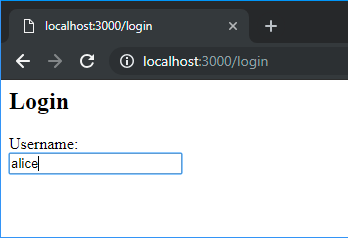
\includegraphics[scale=\myscale]{facetbook_images/10_login.png}};
\node (dash)  at (1, 0)    [draw] {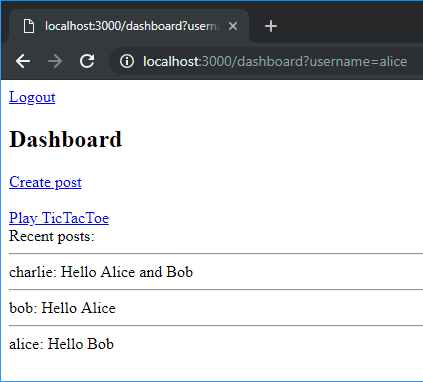
\includegraphics[scale=\myscale]{facetbook_images/11_dashboard.png}};
\node (post)  at (2, -0.1) [draw] {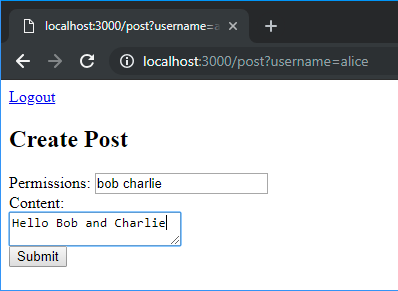
\includegraphics[scale=\myscale]{facetbook_images/12_post.png}};
\node (ttt1)  at (1, 1)    [draw] {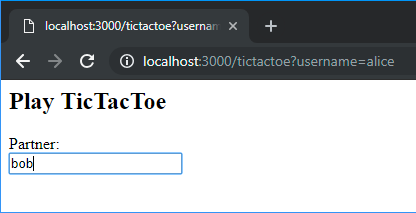
\includegraphics[scale=\myscale]{facetbook_images/13_tictactoe_selectpartner.png}};
\node (ttt2)  at (2, 1)    [draw] {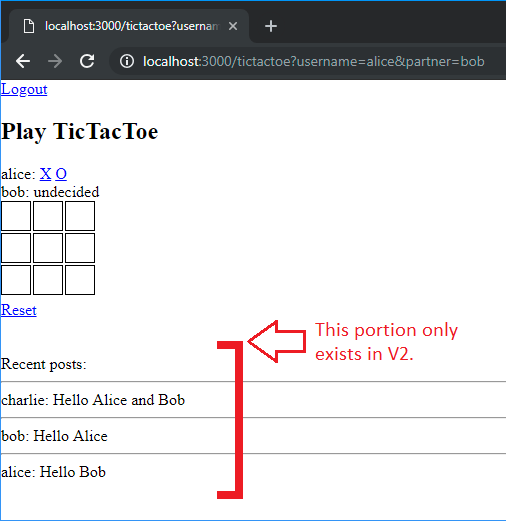
\includegraphics[scale=\myscale]{facetbook_images/14_tictactoe_play.png}};
\draw [->]
  (login) edge (dash)
  (dash)  edge (post)
  (dash)  edge (ttt1)
  (ttt1)  edge (ttt2)
  ;
\end{tikzpicture}
\caption{Screenshots of \myapp{}.}
\label{screenshots}
\end{center}
\end{sidewaysfigure}

The \t{login} page allows typing a username and clicking the ``Submit'' button to go to the \t{dashboard} page.
%
For simplicity, authentication always succeeds with no password required---sophisticated
authentication machinery would remain constant throughout all six versions of \myapp{},
and so would simply add a constant number of lines of code to the TCB.
%
Unlike other work \cite{cecchetti2017nonmalleable},
we make no attempt here to remove authentication code (i.e. password-checking code) from the TCB.

The \t{dashboard} page shows a list of 20 recent posts created by users of \myapp{}.
%
The list comes from the server's database of all posts,
but contains only those that the currently authenticated user is permitted to view.
%
The page also has two links:
one going to the \t{post} page and one to the \t{tictactoe} page.

The \t{post} page allows users to compose posts, and so has a form with two fields:
the \t{permissions} field expects a space-delimited list of usernames indicating who is allowed to see the post,
and the \t{content} field expects any string.
%
Upon clicking ``Submit,'' the form is submitted via HTTP POST protocol to the \t{/post} endpoint,
and the server saves the submitted data in a database.

The \t{tictactoe} page initially shows a form with a single field \t{partner} expecting the username of the person with whom to play Tic Tac Toe.
%
Upon clicking ``Submit,'' the Tic Tac Toe board and its controls appear on the page.
%
If this pair of users
(the currently authenticated user and the specified \t{partner})
has never played Tic Tac Toe together before,
then the server begins by adding a fresh game to the list of ongoing games in the database.
%
Then the server retrieves the game
(whether freshly-created or pre-existing)
from the database and renders it into HTML when serving the page.
%
Thereafter, if the user clicks on the controls of the game,
then the web browser sends a request (using Javascript) specifying what action to take,
and the server updates the game in the database as appropriate.
%
Then the server replies with updated HTML,
which replaces (using Javascript) the display in the browser.

\subsection{Information security}

In \myapp{}, restricted information arrives via HTTP POST protocol at the \t{/post} endpoint.
%
This endpoint is how users express their information flow desires,
namely that only the users specified in the \t{permissions} field can know about this post and its content (in the \t{content} field).

The restricted output channel is the server's response to any incoming HTTP request---unless
that request contains credentials of an appropriate user.
%
In \myapp{}, requests specify credentials in the HTTP GET parameter \t{username}
(rather than in a cookie).

These information security specifications implicitly define a specific attacker model that considers some potential attacks and ignores others.
%
Notably, our model ignores the correctness of the user interface,
which is important because we intend to place the client code in the UCB.
%
If an attacker controls the UCB,
then the attacker could interfere with the creation of the POST request by,
for instance, adding an extra entry to the \t{permissions} field before submitting the POST request.
%
In the design of \myapp{},
we explicitly ignore such an attack and choose instead to assume that the POST parameters received at the server correctly reflect the user's intentions.

\section{FIO library}

Figure \ref{code_fio} shows the interface of the FIO library.
\begin{figure}
\begin{fbstart}
class Lattice a where
  leq :: a -> a -> Bool
  lub :: a -> a -> a
  bot :: a

data Fac l a where
  Undefined :: Fac l a
  Raw       :: a -> Fac l a
  Fac       :: l -> Fac l a -> Fac l a -> Fac l a
  BindFac   :: Fac l a -> (a -> Fac l b) -> Fac l b

data FIORef l a = FIORef (IORef (Fac l a))

data FIO l a where
  Return  :: a -> FIO l a
  BindFIO :: FIO l a -> (a -> FIO l b) -> FIO l b
  Swap    :: Fac l (FIO l a) -> FIO l (Fac l a)
  IO      :: l -> IO a -> FIO l a
  New     :: a -> FIO l (FIORef l a)
  Read    :: FIORef l a -> FIO l (Fac l a)
  Write   :: FIORef l a -> Fac l a -> FIO l ()

data PC l = PC [l] [l]

runFIO :: Lattice l => PC l -> FIO l a -> IO a
\end{fbstart}
\caption{The interface of the FIO library in all versions of \myapp{}.}
\label{code_fio}
\end{figure}
The main difference from previous work \cite{bimonadic} is that this code now supports using an arbitrary security lattice \cite{ngo2018better},
rather than specifically a power set security lattice over the set of \t{String}s.
%
As a result,
the type constructors \t{Fac}, \t{FIORef}, \t{FIO}, and \t{PC} now take an additional type parameter for specifying the security lattice.
%
The corresponding \t{Lattice} type class (lines 1 through 4)
specifies the methods (\t{leq}, \t{lub}, and \t{bot}) that the security lattice must implement.

In addition to the extra type parameter,
we change slightly the representation of the \t{PC} datatype,
so now \t{PC ks1 ks2} denotes the set of lattice elements $k$ such that
\begin{itemize}
  \item
    $k'\sqsubseteq k$ for all $k'\in\t{ks1}$, and
  \item
    $k'\not\sqsubseteq k$ for all $k'\in\t{ks2}$.
\end{itemize}

The main library function is \t{runFIO},
which runs an \t{FIO} computation safely,
namely by respecting the information flow requirements specified by any faceted values used in the computation.
%
The computation bifurcates if necessary.

The FIO library contains 108 lines of code. (Only the interface is shown in Figure \ref{code_fio}.)

\section{\viF}

\myapp{} \viF{} is the initial version of the code,
which implements Design V1,
uses the FIO library,
and is organized so as to minimize the size of the TCB.

\subsection{Tour of TCB}

\subsubsection{Security lattice}

The lattice of security labels is defined in Figure \ref{code_lattice}.
\begin{figure}
\begin{fb}
data Label = Whitelist [User]
           | Bot
instance Lattice Label where
  leq Bot _ = True
  leq _ Bot = False
  leq (Whitelist us1) (Whitelist us2) =
    let subset xs ys = all (\x -> x `elem` ys) xs  in
    us2 `subset` us1
  lub Bot k = k
  lub k Bot = k
  lub (Whitelist us1) (Whitelist us2) =
    Whitelist (List.intersect us1 us2)
  bot = Bot
\end{fb}
\caption{The code for the \t{Label} datatype in all versions of \myapp{}.}
\label{code_lattice}
\end{figure}
The label \t{Bot} is for public data;
the label \t{Whitelist }\textit{users} is for data visible only to the users listed in the list \textit{users}.
%
The datatype \t{Label} forms a lattice,
as evidenced by the type class instance \t{Lattice Label}
and its three methods \t{leq}, \t{lub}, and \t{bot}.

\subsubsection{Database format}

The database format is defined in Figure \ref{code_flist}.
\begin{figure}
\begin{fb}
type Post     = String
data FList a  = Nil
              | Cons a (Fac Label (FList a))
type PostList = FList Post
type Database = (FIORef Label PostList, FIORef Label [TicTacToe])
\end{fb}
\caption{The code for the \t{FList} datatype and associated type definitions in \viF{}.}
\label{code_flist}
\end{figure}
For simplicity, we keep the database in memory rather than on disk
(unlike other work on using faceted values with databases \cite{yang2016precise,alpernas2018secure}).
%
The \t{Database} type is a pair of two mutable references (\t{FIORef}s),
one for holding the current list of posts and a second for holding the current list of ongoing Tic Tac Toe games.
%
The \t{PostList} type makes use of a custom datatype \t{FList},
which is a singly-linked list datatype whose ``next'' pointer is always faceted.
%
The \t{Post} type is simply an alias for Haskell's built-in \t{String} type.

The faceted values in an \t{FList} potentially allow the ``list'' to be structured actually as a tree with branching factor 2.
%
However, in practice, when appending to the list,
each facet shares a suffix with the opposing facet,
so in fact the structure in memory forms a directed acyclic graph whose size is linear in the total number of posts.

\subsubsection{Main function}

Figure \ref{code_main} shows the \t{main} function.
\begin{figure}
\begin{fb}
main :: IO ()
main = do  --IO
  database <- runFIO (Constraints [] []) $ do  --FIO
    r1 <- New Nil
    r2 <- New []
    return (r1, r2)
  let port = 3000
  Warp.run port $ \request respond -> do  --IO
    let (k1, k2) = policy request
    let fio_respond = \x -> IO k2 $ do  --IO
         respond x
         return ()
    let faceted_request = Fac k1 (Raw request) Undefined
    runFIO (Constraints [] []) $
        UCB.handle_request faceted_request database fio_respond
    return ResponseReceived
\end{fb}
\caption{The code for the \t{main} function in \viF{}.}
\label{code_main}
\end{figure}
Its purpose is to start the web server and set up appropriate security sandboxes before handling each request.

Line 47 initializes the database with an empty list of posts,
and line 48 initializes it with an empty list of Tic Tac Toe games.
%
Line 51 creates a socket (using the Haskell library function \t{Warp.run}) for listening for incoming HTTP requests,
which are handled by the code on lines 52 through 59.
%
Line 58 calls \t{UCB.handle\_request}, which is outside the TCB;
however, its inputs (\t{database}, \t{faceted\_request}, and \t{fio\_respond}) are all faceted appropriately,
and its side effects are sandboxed appropriately by \t{runFIO (Constraints [] [])} on line 57.

\subsubsection{Policy function}

The function \t{policy} (called on line 52) computes the appropriate labels to use in \myapp{}.
%
Its code is shown in Figure \ref{code_policy}.
\begin{figure}
\begin{fb}
policy :: WAI.Request -> (Label, Label)
policy request =
  if WAI.pathInfo request == ["login"] then
    (Bot, Bot)
  else case check_credentials request of
    Nothing ->
      (Bot, Bot)
    Just username -> case WAI.pathInfo request of
      ["post"] ->
        let permissions = get_parameter request "permissions"  in
        let users = words permissions  in
        if all valid_username users then
          (Whitelist (username : users), Whitelist [username])
        else
          (Whitelist [username], Whitelist [username])
      _ ->
        (Bot, Whitelist [username])
\end{fb}
\caption{The code for the \t{policy} function in \viF{}.}
\label{code_policy}
\end{figure}
We parse the request to determine its meaning,
and then we return two labels:
one for the confidentiality of the request,
and one for the label of the output channel for returning an HTTP response to the user.

Specifically, this policy assigns \t{Bot} for both labels (lines 63 and 66) when the user is not logged in,
which is the case when requesting the login page (line 62)
or when lacking credentials on any other page (line 65).
%
When the user has valid credentials,
the HTTP response label is \t{Whitelist [username]} (lines 72, 74, and 76),
indicating that the response can contain private information belonging to the authenticated user.
%
For most pages,
the confidentiality label on the request is \t{Bot} (line 76),
which means that the request itself carries no sensitive information;
however, on the \t{"post"} page,
the label \t{Whitelist~(username~:~users)} (line 72) indicates that the request is visible only to
the users named in the \t{permissions} parameter of the request
(and the currently authenticated user too).
%
This label ensures that when the submitted post is written to the database,
it will be faceted appropriately.
%
The label \t{Whitelist [username]} on line 74 is used in case a client sends a malformed request
where the \t{permissions} parameter contains invalid entries.

\subsubsection{Import statements}

The TCB includes the import statements at the top of each file.
\begin{figure}
\begin{fb}
{-# LANGUAGE OverloadedStrings #-}
module UCB where
import qualified Data.List as List
import Data.Monoid((<>))
import Data.String(fromString)
import qualified Data.ByteString.Lazy.Char8 as ByteString(intercalate)
import Network.HTTP.Types.Status(status200, status404)
import qualified Network.Wai as WAI(Request, pathInfo, ResponseLBS)
import Shared
import FIO(FIO(Read, Write, Swap), Fac(), FIORef)
\end{fb}
\caption{The import statements for the \t{UCB} module in \viF{}.}
\label{code_imports_UCB}
\end{figure}
%
\begin{figure}
\begin{fb}
{-# LANGUAGE OverloadedStrings #-}
module Shared where
import Data.String(fromString)
import Data.ByteString.Char8(unpack)
import qualified Network.Wai as WAI(Request, queryString)
import qualified Data.List as List(intersect)
import FIO
\end{fb}
\caption{The import statements for the \t{Shared} module in \viF{}.}
\label{code_imports_Shared}
\end{figure}
%
\begin{figure}
\begin{fb}
{-# LANGUAGE OverloadedStrings #-}
module TCB where
import qualified Network.Wai.Handler.Warp as Warp(run)
import qualified Network.Wai as WAI(Request, pathInfo)
import Network.Wai.Internal(ResponseReceived(ResponseReceived))
import Shared
import FIO
import qualified UCB as UCB(handle_request)
\end{fb}
\caption{The import statements for the \t{TCB} module in \viF{}.}
\label{code_imports_TCB}
\end{figure}
Primarily, we must verify that the \t{UCB} module imports (Figure \ref{code_imports_UCB}) do not include
\t{FIO(runFIO, FIO(IO), Fac(Raw, Fac, Undefined, BindFac))}.
%
As a result, these import statements are actually part of the TCB.

The import statements in the \t{TCB} and \t{Shared} modules are also in the TCB, naturally,
and help auditors determine which standard libraries must be trusted.

\subsubsection{Helper functions}

For completeness, we include the TCB's helper functions,
which are shown in Figure \ref{code_helpers}.
\begin{figure}
\begin{fb}
check_credentials :: WAI.Request -> Maybe User
check_credentials request =
  let username = get_parameter request "username"  in
  if valid_username username  then  Just username
                              else  Nothing

get_parameter :: WAI.Request -> String -> String
get_parameter request key =
  case lookup (fromString key) (WAI.queryString request) of
    Just (Just value) -> unpack value
    _                 -> ""

valid_username :: String -> Bool
valid_username s =
  s /= ""  &&
  all (\c -> (c>='0' && c<='9') ||
             (c>='a' && c<='z') ||
             (c>='A' && c<='Z') ||
             c=='_'                ) s
\end{fb}
\caption{The code for the helper functions in \viF{}.}
\label{code_helpers}
\end{figure}
\t{check\_credentials} is the password-checking function.
%
It gets the username from the HTTP GET parameters.
%
For simplicity, it always succeeds without any password.
%
When no username is supplied,
it returns \t{Nothing},
indicating invalid credentials.
%
\t{get\_parameter} extracts an HTTP GET parameter from a request.
%
\t{valid\_username} checks that a string is non-empty and contains only letters, numbers, and underscores.

\subsubsection{Summary}

In summary, the TCB of \myapp{} \viF{} contains 99 lines: 41 in \t{TCB.hs}, 48 in \t{Shared.hs}, and 10 import statements in \t{UCB.hs}.

\subsection{Tour of UCB}

\subsubsection{Handle-request function}

The entry point to the UCB is \t{handle\_request},
called on line 58 in \t{main}.
%
Figure \ref{code_handle_request} shows its code.
\begin{figure}
\begin{fb}
type Handler = Database -> (WAI.Response -> FIO ()) -> FIO ()
handle_request :: Fac Label WAI.Request -> Handler
handle_request faceted_request database respond = do  --FIO
  Swap $ do  --Fac
    request <- faceted_request
    return $ do  --FIO
      let handler = parse_request request
      handler database respond
  return ()
\end{fb}
\caption{The code for the \t{handle\_request} function in \viF{}.}
\label{code_handle_request}
\end{figure}
Its purpose is to ``unfacet'' the request (i.e. bifurcate if necessary, using \t{Swap} to do so),
and then defer to the helper function \t{parse\_request} and its return value \t{handler} to do the actual processing.
%
At the call site (line 58 in \t{main}),
the faceted request always has a specific shape,
namely with \t{Undefined} in the low-security facet.
%
As a result, the bifurcation at line 124 executes the high-security path like normal (with a changed PC),
and then the low-security path is a no-op.

This code illustrates a typical interaction between the two monads \t{Fac} and \t{FIO}.
%
Line 124 uses \t{Swap} to change the current monad from \t{FIO} to \t{Fac} to allow extracting \t{request} from \t{faceted\_request} on line 125.
%
Then line 126 uses \t{return} to change the current monad back from \t{Fac} to \t{FIO} to allow executing the action on line 128.
%
By using two monads, we can delimit the scope of the bifurcation to be lines 125 to 128.
%
The computations join back together at line 129.

\subsubsection{Parse-request function}

The \t{parse\_request} function translates an incoming web request
(of type \t{WAI.Request}, imported from Haskell's \t{WAI} library for web servers)
into an appropriate action (of type \t{Handler}) to take in response to that request.
%
Figure \ref{code_parse_request} shows its code.
\begin{figure}
\begin{fb}
parse_request :: WAI.Request -> Handler
parse_request request =
  if WAI.pathInfo request == ["login"] then
    login
  else case check_credentials request of
    Nothing ->
      authentication_failed
    Just username -> case WAI.pathInfo request of
      ["post"] ->
        let content = get_parameter request "content"  in
        let permissions = get_parameter request "permissions"  in
        let users = words permissions  in
        if content /= "" && all valid_username users then
          do_create_post username content users
        else
          compose_post username
      ["dashboard"] ->
        dashboard username
      ["tictactoe"] ->
        let partner = get_parameter request "partner"  in
        if valid_username partner then
          let action = get_parameter request "action"  in
          tictactoe_play username partner action
        else
          tictactoe_select_partner username
      _ ->
        not_found
\end{fb}
\caption{The code for the \t{parse\_request} function in \viF{}.}
\label{code_parse_request}
\end{figure}
It duplicates some functionality
(checking whether the request is for the ``login'' page, checking credentials, etc.)
from the \t{policy} function in the TCB,
so it would be reasonable to refactor the code to reduce redundancy.
%
We decided against doing so because the function names \t{policy} and \t{parse\_request} document their purposes well,
whereas it is nontrivial to choose a good name for the newly created functions and intermediate datatypes in the refactored version;
in any case, the amount of duplicated code is small.

\subsubsection{Handler functions}

The \t{parse\_request} function delegates functionality to eight other functions called \t{Handler}s, namely:
\begin{itemize}
  \item
    \t{login}: sends to the client a login page.
  \item
    \t{authentication\_failed}: sends a page to redirect back to the login page.
  \item
    \t{do\_create\_post} \textit{username content users}: inserts a new post into the database and redirects to the dashboard page.
  \item
    \t{compose\_post} \textit{username}: sends to the client a page displaying a form in which the user can compose a new post.
  \item
    \t{dashboard} \textit{username}: sends a page displaying a few links to other pages, as well as a list of recent posts.
  \item
    \t{tictactoe\_play} \textit{username partner action}: updates a Tic Tac Toe game in the database (if necessary)
    and sends to the client a page displaying the current state of the game.
  \item
    \t{tictactoe\_select\_partner} \textit{username}: sends to the client a page prompting the user to type the name of another user.
  \item
    \t{not\_found}: sends a page with ``404 bad request'' on it.
\end{itemize}
The \t{Handler} type is defined on line 121
\[
  \t{type Handler = Database -> (WAI.Response -> FIO ()) -> FIO ()}
\]
and its definition means that it takes as input the database reference cells
(type \t{Database} defined on line 43)
and a callback function (of type \t{WAI.Response -> FIO ()})
whose behavior when called is to send an HTTP response to the user's web browser.
%
Thanks to the code in \t{main},
the database contents are secure (inside \t{FIORef}s)
and the response callback function will not work if the current control flow has been influenced by information that the user should not know
(in that case, the callback would behave as a no-op).

\subsubsection{Summary}

The UCB of \myapp{} \viF{} contains 352 lines: 362 in \t{UCB.hs} minus the 10 import statements at the top of the file,
which are actually part of the TCB.

\section{\viN}

\myapp{} \viN{} is the next version of the code,
which implements Design V1,
does not use the FIO library,
and is organized so as to minimize the size of the TCB.
%
In this section,
we highlight the differences between \viF{} and \viN{}.

\subsection{Removing undesirable dependence on FIO}

The FIO library is unnecessary in this version of \myapp{},
so we can simplify the code by removing dependence on FIO.

First, and most obviously, we remove the file \t{FIO.hs} from the codebase.
%
As a result, we remove all calls to \t{Swap},
which is now unnecessary due to the lack of faceted values.
%
Similarly, we replace uses of \t{New}, \t{Read}, and \t{Write} with uses of \t{newIORef}, \t{readIORef}, and \t{writeIORef}, respectively.
%
Continuing likewise, we remove the \t{FList} datatype (which uses faceted values)
and update the \t{PostList} type definition:
\begin{fb}
type PostList = [(Label, Post)]
\end{fb}
These simple changes affect the line count very little
(aside from removing the 108-line FIO library).

\subsection{Removing desirable dependence on FIO}

Next, we completely remove the \t{policy} function and the lines in \t{main} that depend on it.
%
Figure \ref{code_main_viN} shows the new \t{main} function.
\begin{figure}
\begin{fb}
main :: IO ()
main = do  --IO
  r1 <- newIORef []
  r2 <- newIORef []
  let database = (r1, r2)
  let port = 3000
  Warp.run port $ \request respond -> do  --IO
    let unit_respond = \x -> do  --IO
         respond x
         return ()
    handle_request request database unit_respond
    return ResponseReceived
\end{fb}
\caption{The code for the \t{main} function in \viN{}.}
\label{code_main_viN}
\end{figure}
%
At this point, the functionality of \myapp{} is intact,
but its security guarantees have disappeared---in
particular, all posts are now visible to all users,
regardless of any permission settings on any posts.
%
To reimplement this security feature,
we define a new function \t{filter\_posts}:
\begin{fb}
filter_posts :: Label -> PostList -> PostList
filter_posts k = filter (\(k',p) -> leq k' k)
\end{fb}
and we call it inside the \t{dashboard} function just after reading the posts from the database:
\begin{fb}
labeled_posts <- readIORef (fst database)
let posts = filter_posts (Whitelist [username]) labeled_posts
\end{fb}
We must also add a line to the \t{do\_create\_post} function to label posts just before they are written into the database (line 175):
\begin{fb}
d <- readIORef (fst database)
let labeled_data = ( Whitelist (username : users) ,
                     username ++ ": " ++ content  )
writeIORef (fst database) (labeled_data : d)
\end{fb}

\subsection{Minimizing the TCB}

With only the changes mentioned so far,
the file \t{UCB.hs} is poorly named because it now contains code that belongs in the TCB.
%
To rectify this situation,
we begin by moving four functions from \t{UCB.hs} to \t{TCB.hs},
namely \t{handle\_request}, \t{parse\_request}, \t{do\_create\_post}, and \t{dashboard}.
%
Finally, to keep the TCB as small as possible,
we must rewrite \t{parse\_request} so that it uses sandboxing for the other six types of request (besides \t{do\_create\_post} and \t{dashboard}).
%
The new code is in Figure \ref{code_parse_request_viN}.
\begin{figure}
\begin{fb}
parse_request request =
  let sandbox h = \database respond ->
       let censored = (undefined, snd database)  in
       h censored respond  in
  if WAI.pathInfo request == ["login"] then
    sandbox $ UCB.login
  else case check_credentials request of
    Nothing ->
      sandbox $ UCB.authentication_failed
    Just username -> case WAI.pathInfo request of
      ["post"] ->
        let content = get_parameter request "content"  in
        let permissions = get_parameter request "permissions"  in
        let users = words permissions  in
        if content /= "" && all valid_username users then
          do_create_post username content users
        else
          sandbox $ UCB.compose_post username
      ["dashboard"] ->
        dashboard username
      ["tictactoe"] ->
        let partner = get_parameter request "partner"  in
        if valid_username partner then
          let action = get_parameter request "action"  in
          sandbox $ UCB.tictactoe_play username partner action
        else
          sandbox $ UCB.tictactoe_select_partner username
      _ ->
        sandbox $ UCB.not_found
\end{fb}
\caption{The code for the \t{parse\_request} function in \viN{}.}
\label{code_parse_request_viN}
\end{figure}
Line 179 defines the \t{sandbox} function,
which simply arranges for the posts to be censored from the database before calling a given handler \t{h}.
%
By calling it on lines 182, 185, 194, 201, 203, and 205,
we avoid the need to move any more functions from \t{UCB.hs} to \t{TCB.hs}.

\subsubsection{Summary}

In \viN{}, the TCB contains 118 lines of code:
63 in \t{TCB.hs},
45 in \t{Shared.hs},
and 10 import statements in \t{UCB.hs}.
The UCB contains 295 lines of code:
305 in \t{UCB.hs} minus the 10 import statements at the top of the file.

Qualitatively comparing \viF{} to \viN{} is largely subjective.
%
The application-specific TCB is smaller in \viF{};
on the other hand,
since FIO is part of the TCB,
the total TCB size is less in \viN{}.

Furthermore, the TCB code is qualitatively different in the two implementations.
%
In \viF, the structure of the TCB (especially the \t{policy} function)
relieves auditors from digging through the codebase to find and verify security-critical operations,
such as filtering the list of posts before displaying it,
and correctly labeling new posts before inserting them into the database.
%
On the other hand,
one can argue that the \t{policy} function complicates the control flow.
The control flow in \viN{} is more straightforward,
since there is no need to parse the request twice.

\section{Design V2: Adding a widget}

Design V2 is the same as Design V1 except that the \t{tictactoe} page should now also display recent posts below the Tic Tac Toe game board.
%
Figure \ref{screenshots} highlights the design change in the screenshot of the \t{tictactoe} page.

This design change affects the information flow of \myapp{} because the \t{tictactoe} page now includes information from both portions of the database:
the posts and the games.

\section{\viiF}

\myapp{} \viiF{} implements Design V2,
uses the FIO library,
and is organized so that the change from V1 to V2 is as convenient as possible.

Figures \ref{code_tictactoe_viF} and \ref{code_tictactoe_viiF} show the differences between \viF{} and \viiF{}.
\begin{figure}
\begin{fb}
respond $ WAI.responseLBS status200 headers $
    render_tictactoe new_game username partner
\end{fb}
\caption{Excerpt of the code to display a Tic Tac Toe game in \viF{}.}
\label{code_tictactoe_viF}
\end{figure}
\begin{figure}
\begin{fb}
d <- Read (fst database)
Swap $ do  --Fac
  all_posts <- flatten d
  return $ do  --FIO
    respond $ WAI.responseLBS status200 headers $
        render_tictactoe new_game username partner <>
        "<br /><br />Recent posts:<hr />" <>
        ByteString.intercalate "<hr />" (map escape (take 20 all_posts))
return ()
\end{fb}
\caption{The new code to display a Tic Tac Toe game in \viiF{}.}
\label{code_tictactoe_viiF}
\end{figure}
Only these lines must change to implement the new widget.

In \viiF{}, the TCB is the same as in \viF{}.
%
The UCB contains 8 more lines of code.

Since the TCB is the same in \viF{} and \viiF{},
no further changes are needed to minimize the TCB,
which suggests that the information security is no worse than it was before.
%
Furthermore, no special effort is required to maintain confidence in security when making the change from Design V1 to Design V2.

\section{\viiN}

\myapp{} \viiN{} implements Design V2 without using the FIO library,
and is organized so that the change from V1 to V2 is as convenient as possible.

Figures \ref{code_tictactoe_viN} and \ref{code_tictactoe_viiN} show the differences between \viN{} and \viiN{}.
\begin{figure}
\begin{fb}
respond $ WAI.responseLBS status200 headers $
    render_tictactoe new_game username partner
\end{fb}
\caption{Excerpt of the code to display a Tic Tac Toe game in \viN{}.}
\label{code_tictactoe_viN}
\end{figure}
\begin{figure}
\begin{fb}
labeled_posts <- readIORef (fst database)
let d = filter_posts (Whitelist [username]) labeled_posts
let posts = flatten d
respond $ WAI.responseLBS status200 headers $
    render_tictactoe new_game username partner <>
    "<br /><br />Recent posts:<hr />" <>
    ByteString.intercalate "<hr />" (map escape (take 20 posts))
\end{fb}
\caption{The new code to display a Tic Tac Toe game in \viiN{}.}
\label{code_tictactoe_viiN}
\end{figure}
Aside from these changes,
we must also remove the call to \t{sandbox} on line 202,
which ruins the carefully audited boundary between the TCB and UCB.
%
As a result, in \viiN{}, the file \t{UCB.hs} is poorly named because its contents must now be audited for information leaks.
%
The TCB includes the whole codebase: 429 lines of code.

Note that \viiN{} is still secure (thanks to the call to \t{filter\_posts} on line 221),
just like all the other versions of \myapp{};
however, the auditing effort to confirm its information security increased significantly when we removed the call to \t{sandbox} on line 202.

\section{\viiNm}

\myapp{} \viiNm{} implements Design V2 without using the FIO library,
and is organized so as to minimize the size of the TCB.
%
In this section, we highlight the differences from \viiN{}.

To minimize the TCB,
we must move the \t{tictactoe\_play} function from \t{UCB.hs} to \t{TCB.hs}.
%
To keep the TCB as small as possible,
we also refactor it to call three new functions:
\t{UCB.tictactoe\_error\_response}, \t{UCB.update\_game}, and \t{UCB.tictactoe\_play\_response}.

Figure \ref{code_tictactoe_play} shows the new code for \t{tictactoe\_play}.
\begin{figure}
\begin{fb}
tictactoe_play username partner action database respond =
  if partner == username then
    respond $ UCB.tictactoe_error_response
  else do  --IO
    let censored_database = (undefined, snd database)
    new_game <- UCB.update_game username partner action censored_database
    labeled_posts <- readIORef (fst database)
    let d = filter_posts (Whitelist [username]) labeled_posts
    let posts = flatten d
    respond $ UCB.tictactoe_play_response new_game username partner posts
\end{fb}
\caption{The code for the \t{tictactoe\_play} function in \viiNm{}.}
\label{code_tictactoe_play}
\end{figure}
Lines 231 and 234 set up appropriate sandboxes for calling the UCB functions on lines 232 and 236,
which relieves auditors from reading the code in \t{UCB.hs} (aside from its import statements).

Compared to \viN{},
the TCB is 10 lines larger,
which suggests that the change has reduced confidence in the security of the system.
%
Compared to \viiN{},
we modified 4 lines, moved 6 lines, and inserted 7 new lines;
these changes were necessary to minimize the size of the TCB,
suggesting that some nontrivial effort is required to maintain confidence in security.
%
When FIO is unavailable,
the next best sandboxing techniques lead to an inflexible architecture that becomes outdated when requirements change.

\section{Conclusions}

To quantitatively answer the question of whether FIO makes it easier to achieve information security,
we constructed the prototype social network application \myapp{},
and measured the code changes required to add a widget for displaying recent posts alongside the Tic Tac Toe game.

\subsection{Research question 1}

Does FIO help minimize TCB size when coding a secure application?

The FIO library has 108 lines of code,
and the application-specific TCB in \viF{} has 99 lines of code.
%
The application-specific TCB in \viN{} has 118 lines of code.

In terms of total size,
the TCB is smaller in \viN{}.
%
On the other hand,
the code in FIO is not application-specific,
and so the burden of auditing it for correctness can be amortized over many applications.
%
So our results our inconclusive on this question,
as FIO could be considered helpful or not,
depending on one's point of view.

\subsection{Research question 2}
Does FIO help minimize TCB size when changing an existing application to meet new requirements?

In the FIO version of \myapp{}, the feature extension requires no significant refactoring:
\begin{itemize}
  \item
    We merely add code for getting the posts and displaying them in a widget.
    %
    The extension adds 0 lines of code to the TCB,
    and no special refactoring is required.
\end{itemize}
On the other hand, in the non-FIO codebase,
we have two unappealing options:
\begin{itemize}
  \item
    We could simply remove the sandboxing and implement the extension without refactoring any module boundaries.
    %
    By taking this approach, we greatly increase the size of the TCB,
    which now includes all of the code pertaining to Tic Tac Toe,
    including all helper functions:
    419 lines of code altogether.
  \item
    We could carefully refactor the modules so that we only add to the TCB the code related to displaying the new widget;
    the other helper functions can remain outside of the TCB.
    %
    The net result is still a larger TCB (10 more lines) and extra developer effort (17 changes) spent on refactoring.
\end{itemize}
From this experiment,
we conclude that the FIO library makes it possible in some situations to extend the functionality of applications at no extra cost
(in terms of TCB lines and refactoring effort).
%
In comparison, without FIO,
this feature extension either significantly decreases security (via a larger TCB)
or requires additional refactoring effort to mitigate such a decrease.

\section{Discussion}

One design decision is the richness of the security policy.
%
For instance, we could include all of the rules of the Tic Tac Toe game in the policy,
thus enforcing fair and correct playing of the game.
%
However, since the security policy lies within the TCB,
a larger policy means greater difficulty auditing the policy itself for correctness.
%
Therefore, since correct functionality of the Tic Tac Toe game is less important than enforcing post visibility settings,
we choose to include in the policy only the code pertaining to the latter criterion.

Another design choice is whether to make the policy a ``transparent'' wrapper around the functioning system
(analogous to higher-order contracts being projections \cite{findler2006contracts} that do not modify the behavior of correct programs)
or
to integrate the policy into the functioning system itself.
%
For instance, in \myapp{},
the policy code must inspect the request parameters to determine the request's meaning;
should this part of the code be duplicated in the functioning system,
which also needs to determine each request's meaning?
%
We have chosen to duplicate this code,
so there are some similarities in the control flow of functions \t{policy} and \t{parse\_request} (Figures \ref{code_policy} and \ref{code_parse_request}).

\iffalse
This design choice leads directly into the next design choice,
namely how to structure the code for the non-FIO version of \myapp{},
where the module decomposition is not strictly necessary for separating policy code from everything else.
%
To ease comparison between the two versions,
we choose to use the same module decomposition in the non-FIO version too.
%
Combining the code into a single module would slightly reduce the line count,
but the difference is not substantial.
\fi

For the database, we use the FIORef type from our FIO library to keep persistent state in memory.
%
For the list of ongoing Tic Tac Toe games,
the FIORef will never become faceted because that data is public for everyone to see;
however, for the faceted list of posts,
the situation is more complicated.
%
Specifically, since faceted execution works by refusing to update the facets that are forbidden from seeing the effects of the currently executing code,
the data structure must operate in an append-only manner,
lest we degrade performance by creating an exponentially large faceted structure.
%
Some work by Algehed, Russo, and Flanagan \cite{algehed2019optimizing} will address this performance-related limitation of faceted execution.
%
For now, in \myapp{}, we simply use two separate FIORefs:
one for the list of Tic Tac Toe games (a non-faceted, non-append-only data structure),
and one for the list of posts (a faceted, append-only data structure).



\printbibliography

\end{refsection}
